\documentclass[xcolor={dvipsnames}]{beamer}
\usepackage{color, colortbl}
\usepackage[ngerman,english]{babel}
\usepackage[T1]{fontenc}
\usepackage{CJKutf8} %japanese
\usepackage{lmodern}
\usepackage[compatibility=false]{caption}
\usepackage{subcaption}
\usepackage{tikz}
\usepackage{textgreek}
\usepackage{tabularx}
\usepackage{booktabs}
\usepackage{siunitx}
\usepackage{appendixnumberbeamer}
\usepackage[absolute,overlay]{textpos} %for positioning the logos where I want

\usepackage{animate}
\usepackage{multimedia}

\mode<presentation>
{
  \usetheme{CambridgeUS}     
  \usecolortheme{lily} 
  \definecolor{beamer@violet}{rgb}{0.5,0.3,0.5} % changed this
  \setbeamercolor{structure}{fg=beamer@violet!70!cyan}
  \setbeamercolor{palette primary}{fg=black, bg=gray!30!white!50!cyan!20!}
  \setbeamercolor{palette secondary}{fg=black, bg=gray!30!white!30!cyan!40!}
  \setbeamercolor*{palette tertiary}{bg=gray!20!white!20!cyan!60!}
  
  \setbeamercolor{frametitle}{fg=cyan!60!white!40!,bg=cyan!80!black}
  \setbeamercolor{title}{fg=cyan!80!black}
  \setbeamercolor{normal text}{fg=black,bg=white}
  \setbeamercolor{alerted text}{fg=beamer@violet}
  \setbeamercolor{example text}{fg=beamer@violet!70!cyan}
  
  \usefonttheme{structureitalicserif} 
  \setbeamertemplate{navigation symbols}{}
  \setbeamertemplate{caption}[numbered]
}
\newcommand{\sidlogo}{
  \setlength{\TPHorizModule}{1pt}
  \setlength{\TPVertModule}{1pt}
   % textblock{}{x,y}: pos(x) = rightUpperCorner + (x * \TPHorizModule), pos(y) = leftUpperCorner - (y * \TPVertModule)
  \begin{textblock}{1}(323,12)
   \includegraphics[width=40pt,height=26pt]{figures/SiD.jpeg}
  \end{textblock}
  } 
\newcommand{\ilclogo}{
  \setlength{\TPHorizModule}{1pt}
  \setlength{\TPVertModule}{1pt}
   % textblock{}{x,y}: pos(x) = rightUpperCorner + (x * \TPHorizModule), pos(y) = leftUpperCorner - (y * \TPVertModule)
  \begin{textblock}{1}(323,12)
   \includegraphics[width=40pt,height=26pt]{figures/ILC.jpeg}
  \end{textblock}
} 
\newcommand{\atflogo}{
  \setlength{\TPHorizModule}{1pt}
  \setlength{\TPVertModule}{1pt}
   % textblock{}{x,y}: pos(x) = rightUpperCorner + (x * \TPHorizModule), pos(y) = leftUpperCorner - (y * \TPVertModule)
  \begin{textblock}{1}(323,12)
   \includegraphics[width=40pt,height=26pt]{figures/ATF_logo.jpg}
  \end{textblock}
}
\newcommand{\flukalogo}{
  \setlength{\TPHorizModule}{1pt}
  \setlength{\TPVertModule}{1pt}
   % textblock{}{x,y}: pos(x) = rightUpperCorner + (x * \TPHorizModule), pos(y) = leftUpperCorner - (y * \TPVertModule)
  \begin{textblock}{1}(315,12)
   \includegraphics[width=60pt,height=26pt]{figures/fluka_logo.png}
  \end{textblock}
} 
\newcommand{\ejadelogo}{
  \setlength{\TPHorizModule}{1pt}
  \setlength{\TPVertModule}{1pt}
   % textblock{}{x,y}: pos(x) = rightUpperCorner + (x * \TPHorizModule), pos(y) = leftUpperCorner - (y * \TPVertModule)
  \begin{textblock}{1}(323,12)
   \includegraphics[width=40pt,height=26pt]{figures/EJADE.jpeg}
  \end{textblock}
} 
\newcommand{\BDSsymbol}{
  \setlength{\TPHorizModule}{1pt}
  \setlength{\TPVertModule}{1pt}
   % textblock{}{x,y}: pos(x) = rightUpperCorner + (x * \TPHorizModule), pos(y) = leftUpperCorner - (y * \TPVertModule)
  \begin{textblock}{1}(0,39)
   \includegraphics[width=60pt,height=40pt]{figures/Highlight_BDS.png}
  \end{textblock}
} 
\newcommand{\EXTsymbol}{
  \setlength{\TPHorizModule}{1pt}
  \setlength{\TPVertModule}{1pt}
   % textblock{}{x,y}: pos(x) = rightUpperCorner + (x * \TPHorizModule), pos(y) = leftUpperCorner - (y * \TPVertModule)
  \begin{textblock}{1}(0,39)
   \includegraphics[width=60pt,height=40pt]{figures/Highlight_EXT.png}
  \end{textblock}
} 


\title[ILC \& Background Simulations]{\textbf{\alert{Mini-Workshop on ILC Infrastructure and CFS for Physics and Detectors} \\\LARGE The International Linear Collider \\ \normalsize IP Background Simulations}}
\author{\textbf{Anne Sch\"utz}}
\institute{\textbf{KIT, DESY}}
\date{\textbf{15. March 2016}}

\titlegraphic{\includegraphics[height=1.0cm]{figures/KIT.png}\hspace*{6cm}~%
   \includegraphics[height=1.2cm]{figures/DESY_Logo.png}
}

\begin{document}

{
\usebackgroundtemplate{
 \tikz\node[opacity=0.1]{\includegraphics[width=\paperwidth]{figures/Iwatecomics.jpg}};
 % \tikz\node[opacity=0.2]{\centering\includegraphics[height=\paperheight]{figures/Iwatecomics.jpg}};
 }
\begin{frame}
  \titlepage
\end{frame}
}

\begin{frame}{Table of contents}
  \tableofcontents
\end{frame}


\section{The International Linear Collider}

\subsection{The layout}
\begin{frame}{The layout of the ILC}
\ilclogo
\begin{center}
\only<1>{
\includegraphics[width=\textwidth]{figures/ILC_schematic_layout.png}
}
\only<2->{
\includegraphics[width=\textwidth]{figures/ILC_schematic_layout_centralregion.png}
}
\end{center}
\end{frame}

\section{Background simulation}

\subsection{Background sources}
\begin{frame}{Background sources}
\ilclogo
The main sources of background:
\vspace*{0.5cm}
\begin{columns}
 \begin{column}{0.55\textwidth}
 \only<1>{
  \begin{itemize}
    \item Pair background
    \item Bhabha scattering
    \item \textgamma \textgamma $\rightarrow$ hadrons
    \item Neutrons from the beam dumps
    \item Background from Final-Focus system
    \begin{itemize}
     \item Beam halo collimators
     \item Muon spoilers
    \end{itemize}
  \end{itemize}
  }
  \only<2>{
  \begin{itemize}
    \item \alert{\MakeUppercase{Pair background}}
    \item \alert{Bhabha scattering}
    \item \alert{\textgamma \textgamma $\rightarrow$ hadrons}
    \item Neutrons from the beam dumps
    \item Background from Final-Focus system
    \begin{itemize}
     \item Beam halo collimators
     \item Muon spoilers
    \end{itemize}
  \end{itemize}
  }
 \only<3>{
  \begin{itemize}
    \item Pair background
    \item Bhabha scattering
    \item \textgamma \textgamma $\rightarrow$ hadrons
    \item \alert{\MakeUppercase{Neutrons from the beam dumps}}
    \item Background from Final-Focus system
    \begin{itemize}
     \item Beam halo collimators
     \item Muon spoilers
    \end{itemize}
  \end{itemize}
  }
  \only<4>{
  \begin{itemize}
    \item Pair background
    \item Bhabha scattering
    \item \textgamma \textgamma $\rightarrow$ hadrons
    \item Neutrons from the beam dumps
    \item \alert{Background from Final-Focus system}
    \begin{itemize}
     \item \alert{\MakeUppercase{Beam halo collimators}}
     \item \alert{Muon spoilers}
    \end{itemize}
  \end{itemize}
  }
   \only<5>{
  \begin{itemize}
    \item Pair background
    \item Bhabha scattering
    \item \textgamma \textgamma $\rightarrow$ hadrons
    \item Neutrons from the beam dumps
    \item \alert{Background from Final-Focus system}
    \begin{itemize}
     \item \alert{Beam halo collimators}
     \item \alert{\MakeUppercase{Muon spoilers}}
    \end{itemize}
  \end{itemize}
  }
 \end{column}
 \begin{column}{0.45\textwidth}
 \only<2>{
 \includegraphics[height=0.2\textheight]{figures/beamstrahlung_processes.png}\\
 \includegraphics[height=0.15\textheight]{figures/bhabha_scattering.pdf} 
 \includegraphics[height=0.15\textheight]{figures/gammagamma_hadrons.pdf}
 }
 \only<3>{
 \includegraphics[height=0.45\textheight]{figures/FLUKA_quadrupole_model.png}
 }
 \only<4>{
 \includegraphics[height=0.45\textheight]{figures/ATF2_beamhalo_collimator.pdf}
 }
 \only<5>{
 \includegraphics[height=0.45\textheight]{figures/Muons.png}
 }
 \end{column}
\end{columns}

\end{frame}

\subsection{Simulation tools}
\begin{frame}{Simulation tools}
Simulation tools used for the studied background sources:
\vspace*{0.5cm}
  \begin{itemize}
    \item Pair background - \alert{GuineaPig}
    \item Bhabha scattering - \alert{Pythia}
    \item \textgamma \textgamma $\rightarrow$ hadrons - \alert{Pythia}
    \item Neutrons from the beam dumps - \alert{FLUKA}
    \item Beam halo collimators - \alert{BDSIM}
    \item Muon spoilers - \alert{MUCARLO}
  \end{itemize}
\end{frame}

\subsection{Pair background in the SiD detector}
\begin{frame}
 \begin{center}
  \alert{\MakeUppercase{Pair background}}
 \end{center}
\end{frame}

\begin{frame}{SiD detector}
\sidlogo
\begin{figure}[T]
\centering
\begin{subfigure}[b]{0.49\textwidth}
\centering
\includegraphics[height=0.65\textheight]{figures/SiD_detector_model.pdf}
\end{subfigure}
\begin{subfigure}[b]{0.49\textwidth}
\centering
\includegraphics[height=0.65\textheight]{figures/SiD_detector_model_Ausschnitt.pdf}
\end{subfigure}
\caption{\small SiD detector model: Vertex detector (red), ECAL (green), HCAL (pink), Muon system (blue)}
\end{figure}
\end{frame}

\begin{frame}{Pair background}
\sidlogo
 \begin{figure}
 	\begin{columns}
        \column[T]{0.75\linewidth} 
        \begin{flushright}
        \includegraphics[height=0.55\textheight]{figures/sidloi3_pairs_1312_EcalEndcap_HitsPerFile_Particles.png}
        \end{flushright}
        \column[T]{0.25\linewidth}
        \begin{flushleft}
        \caption{\small Distribution of number of pair background particles per bunch crossing hitting the detector.}
        \end{flushleft}
      \end{columns}
\end{figure}
Per bunch, there are about \num{200000} pair background particles, in the whole detector.\\
\visible<2->{
\begin{center}
 In comparison:\\
e$^+$e$^-\rightarrow$\,ZH\,$\rightarrow$\,4 jets: $\sim$ 80 final state particles
%e$^+$e$^-\rightarrow$\,W$^+$W$^-$ $\sim$ 1000/hour 
%\hspace*{0.5cm}
%e$^+$e$^-\rightarrow$\,HX $\sim$ 10/hour
\end{center}
}
\end{frame}


\begin{frame}[label=HitsEcalEndcaps]{Hits in the SiD - EcalEndcaps}
\sidlogo
\begin{columns}
\begin{column}[T]{0.5\textwidth}
\begin{figure}
\centering
\includegraphics[width=\textwidth]{figures/sidloi3_pairs_1312_EcalEndcap_HitsPerFile_Hits.png}
\caption{\small Hits of pair background particles from a full train in the EcalEndcaps}
\end{figure}
\end{column}
\begin{column}[T]{0.5\textwidth}
\begin{figure}
\centering
\includegraphics[width=\textwidth]{figures/sidloi3_pairs_1312_EcalEndcap_Hits_EcalEndcap_MeanHits_0-4.png}
\caption{\small Comparison of the MEAN number of hits in the first 5 layers of the EcalEndcaps.}
\end{figure}
\end{column}
\end{columns}
In the EcalEndcaps only, there are about 200 hits per bunch crossing.\\
\only<1>{
\vspace*{0.2cm}
The mean number of hits per layer is between 15 and 25 hits, per full bunch crossing!\\
}
\only<2>{
\vspace*{0.2cm}
\begin{center}
 In comparison:\\
e$^+$e$^-\rightarrow$\,ZH\,$\rightarrow$\,4 jets: $\sim$ \num{2100} hits in the EcalEndcaps
\hyperlink{ZH_event_display}{\beamergotobutton{Go to event display}}
\end{center}
}
\end{frame}

\begin{frame}[t]{3D hit map animation of the EcalEndcaps}
\sidlogo
\begin{center}
\only<1>{
  \animategraphics[portait,autoplay,loop,height=6cm]{2}{figures/3Danimation_EcalEndcap/Hits_3D_EcalEndcap_Layer_}{0}{30}
}
\only<2->{
  \includegraphics[height=6cm]{figures/3Danimation_EcalEndcap/Hits_3D_EcalEndcap_Layer_0.png}
}
\end{center}
Most of the hits are around the beam pipe $\rightarrow$ Ring of fire
\end{frame}

\begin{frame}{Pair background origins}
\sidlogo
  \begin{figure}
 	\begin{columns}
        \column[T]{0.75\linewidth} 
        \begin{flushright}
        \includegraphics[width=0.9\textwidth]{figures/sidloi3_pairs_1312_EcalEndcap_Hits_EcalEndcap_ParticleOrigins_EcalEndcap_Layer_0.pdf}
        \end{flushright}
        \column[T]{0.25\linewidth}
        \begin{flushleft}
	\caption{\small 2D map of the origins of the pair background particles that hit the EcalEndcap layer 0.}
        \end{flushleft}
      \end{columns}
\end{figure}

Most of the background particles are coming from the IP as expected.\\
But there are a lot of particles backscattering from the tracker layers and the BeamCal.
\end{frame}

\subsection{FLUKA simulation of the ILC Beam Dump}
\begin{frame}
 \begin{center}
  \alert{\MakeUppercase{Neutrons from the beam dump}}
 \end{center}
\end{frame}

\begin{frame}{FLUKA simulation of the ILC Beam Dump}
\flukalogo
\EXTsymbol
\begin{columns}[T]
\begin{column}[b]{0.4\textwidth}
 \begin{figure}
 \centering
\includegraphics[height=0.45\textheight]{figures/FLUKA_quadrupole_model.png}
\caption{\small FLUKA simulation model of one of the ILC lattice quadrupoles.}
\end{figure}
\end{column}
\begin{column}[b]{0.6\textwidth}
\begin{itemize}
 \item The beam is dumped into a water tank after collision.
 \item Neutrons are emitted that radiate the surroundings.
 \item Neutrons fly back towards the detectors.
\end{itemize}
\vspace*{0.5cm}
\visible<2->{
\begin{block}{Simulation}
With Benno List (DESY): Pluging the real extraction line lattice into FLUKA.\\
Realistic simulation of the interaction between the neutrons,the lattice and the detectors.
\end{block}
}
\end{column}
\end{columns}
\end{frame}

\subsection{Final-Focus system as a background source}
\begin{frame}
 \begin{center}
  \alert{\MakeUppercase{Background from Beam Halo collimators}}
 \end{center}
\end{frame}

\begin{frame}{Beam Halo collimators}
\BDSsymbol
 \begin{center}
\includegraphics[width=0.65\textwidth]{figures/ATF2_beamhalo_collimator.pdf}
\end{center}
By driving collimator blocks into the beam:\\
\begin{itemize}
 \item The beam halo is cut off.
 \item Wakefields are induced.
 \item New background is produced.
\end{itemize}

\end{frame}
\subsection{ATF2}
\begin{frame}{Accelerator Test Facility 2}
\atflogo
ATF2: Extension of the Accelerator Test Facility (ATF) at KEK
\vspace*{0.3cm}
\begin{center}
 \only<1>{\includegraphics[width=0.7\textwidth]{figures/kek_map.pdf}}
 \only<2->{\includegraphics[width=0.7\textwidth]{figures/kek_map_stars.pdf}}
\end{center}

\end{frame}

\begin{frame}{Accelerator Test Facility 2}
\atflogo
ATF2
\begin{itemize}
\item Test bench for the Final-Focus system of the ILC $\rightarrow$ very close to the ILC 500
\item Achieving \SI{40}{\nano\metre} beam size (goal: \SI{37}{\nano\metre})
\end{itemize}
\vspace*{0.3cm}
\begin{center}
 \includegraphics[width=0.8\textwidth]{figures/ATF.jpg}
\end{center}

\end{frame}

\begin{frame}{Beam time at ATF2 in March}
\ejadelogo
At the moment, I am joining the ATF2 beam time, thanks to the E-JADE program {\tiny(www.e-jade.eu)}.
\begin{itemize}
\item Measuring the background generated by the installed beam halo collimator with Cherenkov detector
\item Simulating the background with BDSIM
\end{itemize}
\begin{columns}[T]
 \begin{column}[t]{0.75\textwidth}
 \flushright
  \includegraphics[width=0.67\textwidth]{figures/rhulcher1_20160311morning_signal_averagesignal_aperture.png}
 \end{column}
 \begin{column}[t]{0.25\textwidth}
  \flushleft
  \textcolor{RubineRed}{FIRST RESULTS}
 \end{column}
\end{columns}
\end{frame}

\subsection{Muon from spoilers}
\begin{frame}
 \begin{center}
  \alert{\MakeUppercase{Muons from spoilers}}
 \end{center}
\end{frame}

\begin{frame}{Muon from spoilers}
 Lewis Keller: MUCARLO simulation of the muon tracks in the BDS tunnel.\\
 4-vectors of muons at IP are available to simulate muons in detectors
 \begin{center}
 	\includegraphics[width=0.7\textwidth]{figures/Muons.png}
  \end{center}
\end{frame}

\begin{frame}{Muons at IP}
Number of the muons at the IP
  \begin{center}
 	\includegraphics[width=0.9\textwidth]{figures/mucarlo_numbers.pdf}
  \end{center}
\end{frame}

\section*{Summary}
\begin{frame}{Summary}
Current effort in simulating the background at the IP:
 \begin{itemize}
  \item Background from beam-beam interactions
  \item Neutron background from the beam dump
  \item Muon background from spoilers
 \end{itemize}
 
 \vspace*{0.5cm}
 
 \begin{center}
  \includegraphics[width=0.6\textwidth]{figures/ILC_LHC_eventdisplay_comparison.pdf}
 \end{center}


\end{frame}




\section*{The end}
{
\usebackgroundtemplate{
 \tikz\node[opacity=0.1]{\includegraphics[width=\paperwidth,resolution=200]{figures/ilc-Comic.png}};
 % \tikz\node[opacity=0.2]{\centering\includegraphics[height=\paperheight]{figures/Iwatecomics.jpg}};
 }
\begin{frame}
\ilclogo
\begin{center}
\textcolor{RubineRed}{
	\LARGE Thanks!\\
	\vspace*{0.5cm}
	\begin{CJK}{UTF8}{min}
	どうもありがとうございます。
	\end{CJK}
}
\end{center}
\end{frame}
}

\section*{References}
\begin{thebibliography}{9}
\begin{frame}{References}
\bibitem{TDR} T. Behnke, et al. \emph{The International Linear Collider - Technical Design Report}, 2013.
\bibitem{RHUL} Mark Thomson. \emph{Physics and Detectors at the ILC}, 2013. \url{https://www.royalholloway.ac.uk/physics/documents/pdf/events/particlephysicsseminars/13-14markthomson23oct2013.pdf}
\bibitem{ATF2} Kuroda et al. \emph{A plan of KEK-ATF Final Focus Test Beam Line (ATF2)
}. \url{http://icfa-nanobeam.web.cern.ch/icfa-nanobeam/paper/urakawa_ATF2-2.pdf}
\bibitem{Collimator} N. Fuster-Martínez, IFIC (CSIC-UV), et al. \emph{Design study and construction of a transverse Beam Halo Collimation system for ATF2}, 2015. \url{http://accelconf.web.cern.ch/AccelConf/IPAC2015/papers/wepmn059.pdf}
\bibitem{Muons} Lew Keller (SLAC)

\end{frame}
\end{thebibliography}

%--------------------------------------------------------------------------------
\appendix

\begin{frame}
\begin{center}
\LARGE Additional Material
\end{center}
  \tableofcontents
\end{frame}

\section{ILC}

\subsection{Some facts about the SiD detector}
\begin{frame}{SiD detector}
\sidlogo
 \begin{columns}
  \begin{column}{0.7\textwidth}
    SiD has a very convincing design:
 \begin{itemize}
  \item compact and robust
  \item full silicon vertex detector and tracker\\
  Vertex detector:
  \begin{itemize}
   \item $<$\SI{5}{\micro\metre} resolution
   \item Momentum resolution $\sim$ 2-\SI{5e-5}{\per\giga\electronvolt}
   \item $\sim$ \SI{0.1}{\percent} X$_0$ per layer
    \item Single bunch timing resolution
    \item cos($\theta$)$\approx$0.984
  \end{itemize}
  \item highly granular calorimetry optimized for Particle Flow (ECAL: radation length = 26 X$_0$, \\EM energy resolution = 0.17/$\sqrt{E}\bigoplus$1\%)
 \end{itemize}
  \end{column}
  \begin{column}{0.3\textwidth}
    \begin{flushright}
  \includegraphics[height=0.4\textheight]{figures/SiDpics.pdf}
 \end{flushright}
  \end{column}
 \end{columns}

\end{frame}

\section{Additional SiD simulation plots}

\subsection{Higgs event display}
\begin{frame}[label=ZH_event_display]{e$^+$e$^-\rightarrow$\,ZH\,$\rightarrow$\,4 jets in the SiD detector}
e$^+$e$^-\rightarrow$\,ZH\,$\rightarrow$\,4 jets in the SiD detector\\
Displayed with WIRED4
 \begin{center}
   \includegraphics[width=0.8\textwidth]{figures/Zhiggs_4jets_SiD.png}\\
 \hyperlink{HitsEcalEndcaps}{\beamergotobutton{Go back}}
 \end{center}
\end{frame}

\subsection{Hit maps of the EcalEndcap}
\begin{frame}{Hit maps of the inner most EcalEndcap layer}
\sidlogo
\begin{columns}[T]
\begin{column}[b]{0.5\textwidth}
 \begin{figure}
\centering
\includegraphics[height=0.5\textheight]{figures/sidloi3_pairs_1312_EcalEndcap_Hits_EcalEndcap_Hits_2D_EcalEndcap_Layer_0-eps-converted-to.pdf}
\caption{\small 2D hit map of the hits from a full pair background train in the EcalEndcap layer 0.}
\end{figure}
\end{column}
\begin{column}[b]{0.5\textwidth}
 \begin{figure}
\centering
\includegraphics[height=0.5\textheight]{figures/Hits_3D_EcalEndcap_Layer_0.png}
\caption{\small 3D hit map of the hits from a full pair background train in the EcalEndcap layer 0.}
\end{figure}
\end{column}
\end{columns}
Most of the hits are around the beam pipe $\rightarrow$ Ring of fire
\end{frame}

\subsection{Absolute time of hits}
\begin{frame}{Absolute time of hits in the EcalEndcaps}
\sidlogo
\only<1>{
\begin{figure}
\centering
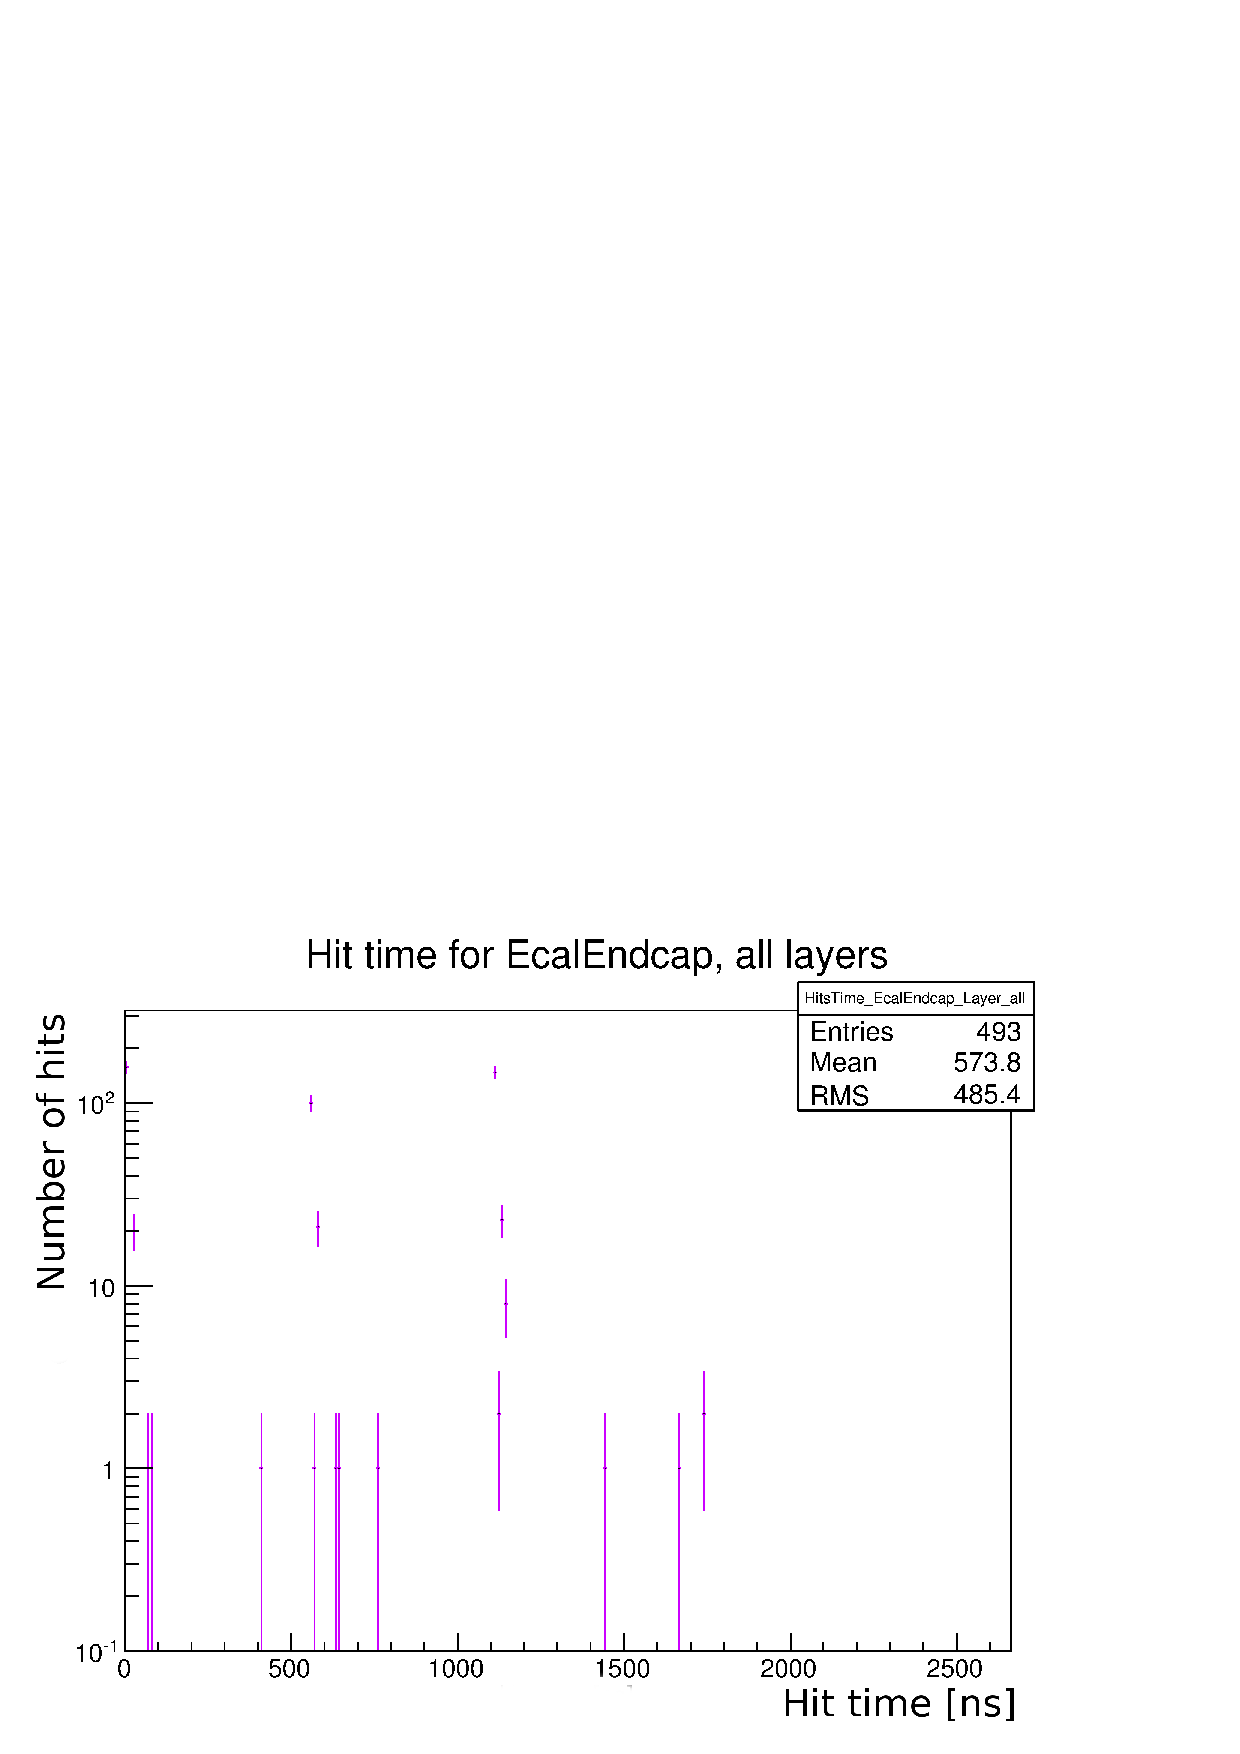
\includegraphics[height=0.55\textheight]{figures/3_sidloi3_EcalEndcap_Hits_EcalEndcap_HitsTime_EcalEndcap_Layer_all.pdf}
\caption{\small Number of particles arriving at the EcalEndcaps as a function of the absolute time.}
\end{figure}
}
\only<2>{
\begin{figure}
\centering
\includegraphics[height=0.6\textheight]{figures/3_sidloi3_EcalEndcap_Hits_EcalEndcap_HitsTime_rtime_2D_EcalEndcap_Layer_all-biggerdots.pdf}
\caption{\small The radial position of the particles arriving at the EcalEndcaps.}
\end{figure}
}
The pair background particles don't arrive all at the same time.\\
The second smaller peak of particles are backscatter particles.
\end{frame} 

\subsection{Hit energy deposition}
\begin{frame}{Energy deposition of hits in SiD-EcalEndcaps}
\sidlogo
 \begin{figure}
 \centering
  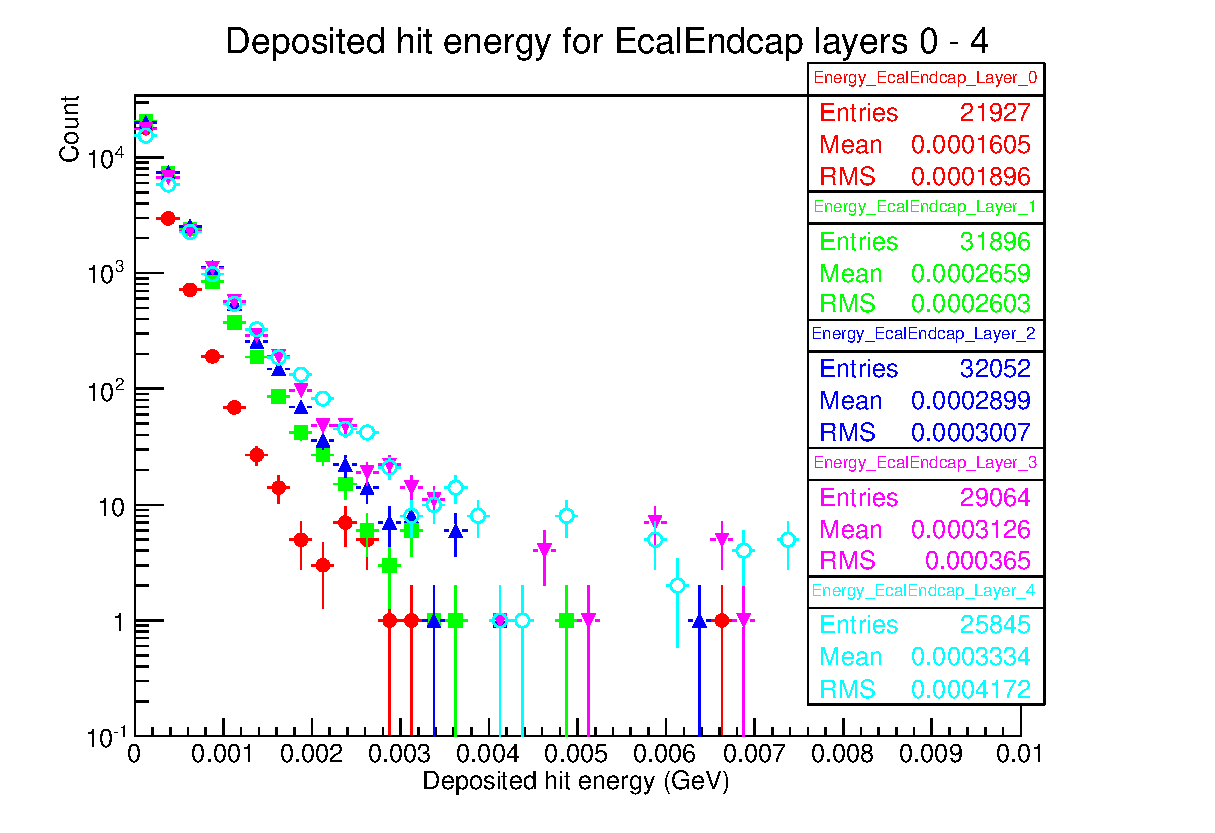
\includegraphics[width=0.6\textwidth]{figures/sidloi3_pairs_1312_EcalEndcap_Hits_EcalEndcap_Energy_EcalEndcap_Layer_0-4.eps}
 \caption{Energy distribution of the hits in the first five layers of the SiD EcalEndcaps}
 \end{figure}
The distributions reach up to about \SI{8}{\mega\electronvolt}.
\end{frame}

\section{The Final-Focus system}
\begin{frame}{The Final-Focus system}
 \ilclogo
 The Final-Focus (FF) uses:
\begin{itemize}
 \item Strong compact superconducting quadrupoles to focus the
beam at the IP (single collision point with a 14 mrad beam-crossing angle)
\item Sextupoles providing local chromaticity correction
\item Two superconducting octupole doublets, which use nonlinear
focusing to reduce the amplitude of beam-halo particles while leaving the beam core untouched $\rightarrow$ permitting larger collimation amplitude
\item Collimators and spoilers to prevent the beam halo and background particles from entering the detectors
\end{itemize}
\end{frame}



\end{document}
